\documentclass{article}
\usepackage[margin=1in]{geometry} % For setting page margins
\usepackage{amsmath}
\usepackage{amssymb} % For math symbols and equations
\usepackage{graphicx} % For including images
\usepackage{hyperref} 
\usepackage{enumitem}
\usepackage{float}
\usepackage{listings}
\usepackage{xcolor}
\usepackage{caption}

\renewcommand{\thesection}{\arabic{section}.}
\renewcommand{\thesubsection}{(\alph{subsection})}

\lstdefinestyle{matlabstyle}{
    language=Matlab,              % Specify the language
    basicstyle=\ttfamily\footnotesize\color{black}, % Code font
    keywordstyle=\color{blue}\bfseries, % Keywords in blue
    stringstyle=\color{orange},    % Strings in green
    commentstyle=\color{magenta}, % Comments in magenta
    numbers=left,                 % Line numbers on the left
    numberstyle=\tiny\color{black},% Line number style
    stepnumber=1,                 % Line number increment
    breaklines=true,              % Line breaking
    frame=single,                 % Border around code
    backgroundcolor=\color{white},
    tabsize=4,                    % Tab size
    showstringspaces=false,       % Don't show spaces in strings
}

\begin{document}

\title{
    \begin{tabular}{@{}l@{}}
        \textbf{Class:} Robust Multivariate Control \\
        \textbf{Professor:} Dr. Sean Humbert \\
        \textbf{TAs:} Santosh Chaganti \\
        \textbf{Student:} Steve Gillet \\
        \textbf{Date:} \today \\
        \textbf{Assignment:} Homework 6
    \end{tabular}
}

\author{}
\date{}

\maketitle

\section{}

\textit{
In this problem you will use $H_\infty$ synthesis techniques to design a roll angle hold control system for a fixed wing UAS with actuator dynamics. The roll dynamics are given by
\[
\begin{aligned}
    \dot{p} &= L_p p + L_{\delta_a} \delta_a, \\
    \dot{\phi} &= p,
\end{aligned}
\]
where $p$ is the roll rate, $\phi$ is the roll angle and $\delta_a$ is the aileron deflection. The stability and control derivatives are $L_p = -1$ and $L_{\delta_a} = 30$. We will assume first order actuator dynamics for the aileron servomotors, hence
\[
\dot{\delta}_a = -\frac{1}{\tau} \delta_a + \frac{1}{\tau} V
\]
where $V$ is the input voltage to the servomotor and $\tau = 0.1$ is the motor time constant.
}

\subsection{}

\textit{Augment the roll dynamics with the actuator dynamics to generate a new state space model for the combined plant $G$ with state $x = [p\ \phi\ \delta_a]^T$ and input $V$.}

The roll dynamics with actuator dynamics are given by:
\[
\begin{aligned}
\begin{bmatrix}
\dot{p} \\
\dot{\phi} \\
\dot{\delta}_a
\end{bmatrix}
&=
\begin{bmatrix}
L_p & 0 & L_{\delta_a} \\
1 & 0 & 0 \\
0 & 0 & -\frac{1}{\tau}
\end{bmatrix}
\begin{bmatrix}
p \\
\phi \\
\delta_a
\end{bmatrix}
+
\begin{bmatrix}
0 \\
0 \\
\frac{1}{\tau}
\end{bmatrix}
V
\end{aligned}
\]

\subsection{}

\textit{Generate a block diagram of the closed loop system assuming our measurement is the roll angle $\phi_r$. We want to have the closed loop system track the roll angle reference $\phi_r$ with actuator limits, so assume performance outputs $z_1 = W_1 e$ and $z_2 = W_2 u$. Be sure to label all the important signal quantities $(z_1, z_2, v, w, u)$ on the block diagram.}

\begin{figure}[H]
    \centering
    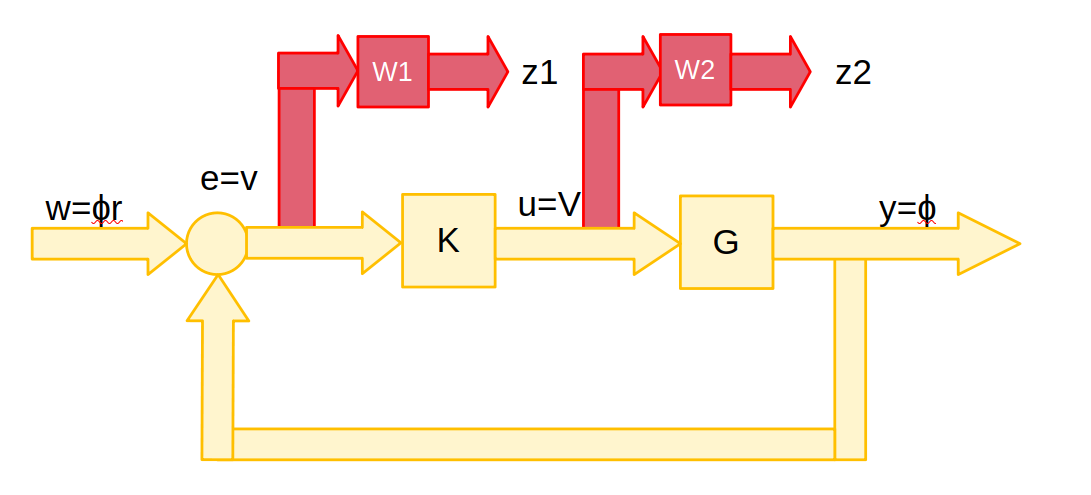
\includegraphics[width=\textwidth]{uasBlock.png}
\end{figure}

\subsection{}

\textit{Compute the generalized plant $P$ and close the lower LFT to compute the corresponding $w \to z$ transfer function and test for $H_\infty$ nominal performance.}

The performance outputs and signals are defined as:
\[
\begin{aligned}
z_1 &= W_1 (w - Gu), \\
z_2 &= W_2 u, \\
v &= e = w - Gu.
\end{aligned}
\]

The generalized plant $P$ is constructed as:
\[
\begin{bmatrix}
z_1 \\
z_2 \\
v
\end{bmatrix}
=
\begin{bmatrix}
W_1 & -W_1 G \\
0 & W_2 \\
I & -G
\end{bmatrix}
\begin{bmatrix}
w \\
u
\end{bmatrix}
\]

The closed-loop transfer function $F_\ell(P, K)$ is derived as:
\[
\begin{aligned}
F_\ell(P, K) &= P_{11} + P_{12} K (I - P_{22} K)^{-1} P_{21}, \\
F_\ell(P, K) &= \begin{bmatrix}
W_1 \\
0
\end{bmatrix}
+ \begin{bmatrix}
-W_1 G \\
W_2
\end{bmatrix}
K (I + G K)^{-1} I, \\
&= \begin{bmatrix}
W_1-W_1 G K (I + G K)^{-1} \\
W_2 K (I + G K)^{-1}
\end{bmatrix} \\
&= \begin{bmatrix}
W_1 (I - T_O) \\
W_2 K S_O
\end{bmatrix} \\
&= \begin{bmatrix}
W_1 S_O \\
W_2 K S_O
\end{bmatrix}
\end{aligned}
\]

The $H_\infty$ performance criteria are:
\[
\| \begin{bmatrix} W_1 S_O \\ W_2 K S_O \end{bmatrix} \|_\infty < 1
\]
where $S_O = (I + G K)^{-1}$ is the sensitivity function.

\subsection{}

\textit{Assume a tracking performance weighting function to be $W_1(s) = (s/M + \omega_B^*)/(s + \omega_B^* A)$ and an actuator usage weighting function (predetermined by the given actuator performance) to be $W_2(s) = 100(s + 0.1)/(s + 100)$. Implement MATLAB code to synthesize a $H_\infty$ controller $K$ using \texttt{hinfyn} and \texttt{sysic}. Your design parameters for tracking are $A$, $M$ and $\omega_B^*$. Ideally the rise time for the closed loop would be less than 4 seconds with minimal steady-state error.}

\begin{lstlisting}[style=matlabstyle]
Lp = -1;
Lda = 30;
tau = 0.1;

A = [Lp 0 Lda; 1 0 0; 0 0 -1/tau];
B = [0; 0; 1/tau];
C = [0 1 0];
D = 0;
G = ss(A,B,C,D);

M = 2;
A = 0.005;
omegaB = 1;

W1 = tf([1/M omegaB], [1 omegaB*A]);
W2 = tf([100 10], [1 100]);

systemnames = 'G W1 W2';
inputvar = '[w; u]';
outputvar = '[W1; W2; w-G]';
input_to_G = '[u]';
input_to_W1 = '[w-G]';
input_to_W2 = '[u]';
sysoutname = 'P';
sysic;
P = minreal(ss(P));

m = size(B,2);
p = size(C,1);
[K, CL, gamma, info] = hinfsyn(P,p,m,'method','ric','Tolgam',1e-3,'DISPLAY','on');     
\end{lstlisting}

\subsection{}

\textit{When you have settled on a sufficient design, verify that your system satisfies nominal performance by plotting the $|1/W_1(j\omega)|$ and $\hat{\sigma}(S_0)$ curves, and the $|1/W_2(j\omega)|$ and $\hat{\sigma}(KS_0)$ curves. Also plot the step response for a unit step input in $\phi_r$.}

\begin{figure}[H]
    \centering
    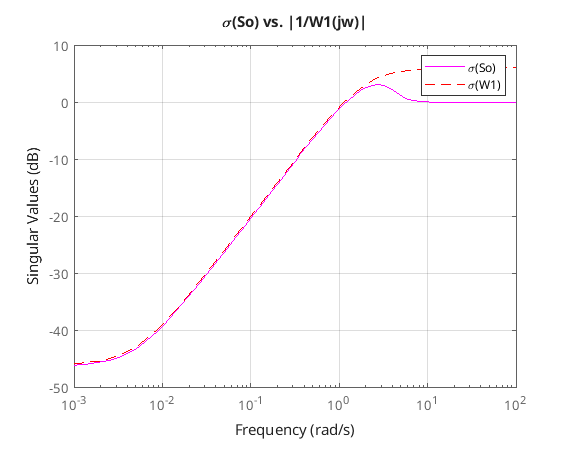
\includegraphics[width=\textwidth]{uasSigmaSo.png}
\end{figure}

\begin{figure}[H]
    \centering
    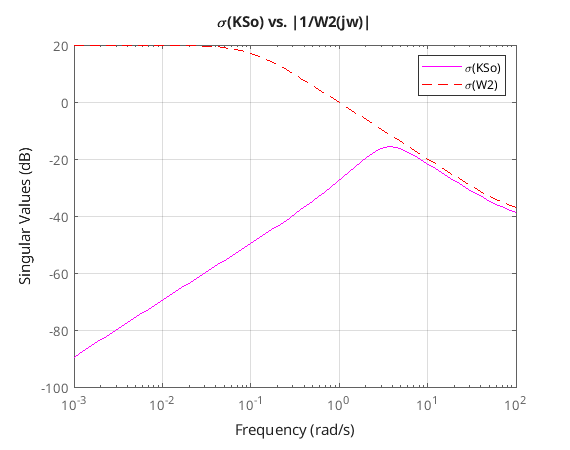
\includegraphics[width=\textwidth]{uasSigmaKSo.png}
\end{figure}

\begin{figure}[H]
    \centering
    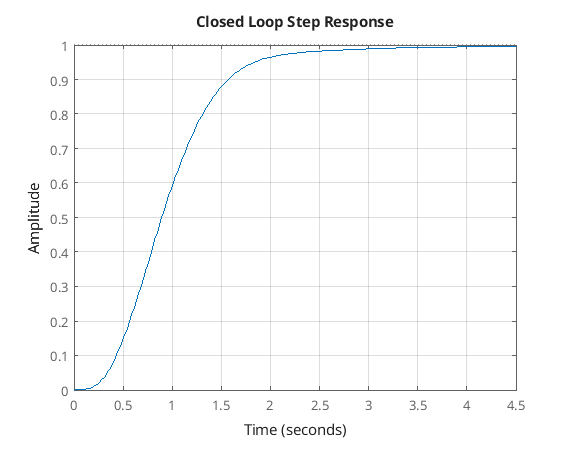
\includegraphics[width=\textwidth]{uasStep.png}
\end{figure}

\section{}
\textit{In this problem you will gain some experience with a MIMO plant by synthesizing a disturbance rejection controller for the lateral dynamics of an A-4 aircraft. The plant has two states, $\beta$ (sideslip angle) and $r$ (yaw rate), along with two control inputs $\delta_a$ (aileron angle) and $\delta_r$ (rudder angle). Assume both states are measurable, i.e., $C = I$. The dynamics are available to download in an m-file from Canvas.}
    
\subsection{}
\textit{Generate a block diagram of the closed loop system assuming an output disturbance $w_1 = d_o \in \mathbb{R}^2$, with a performance output $z = W_p y \in \mathbb{R}^2$. Be sure to label all the important signal quantities $(z, v, w, u)$ on the block diagram.}

\begin{figure}[H]
    \centering
    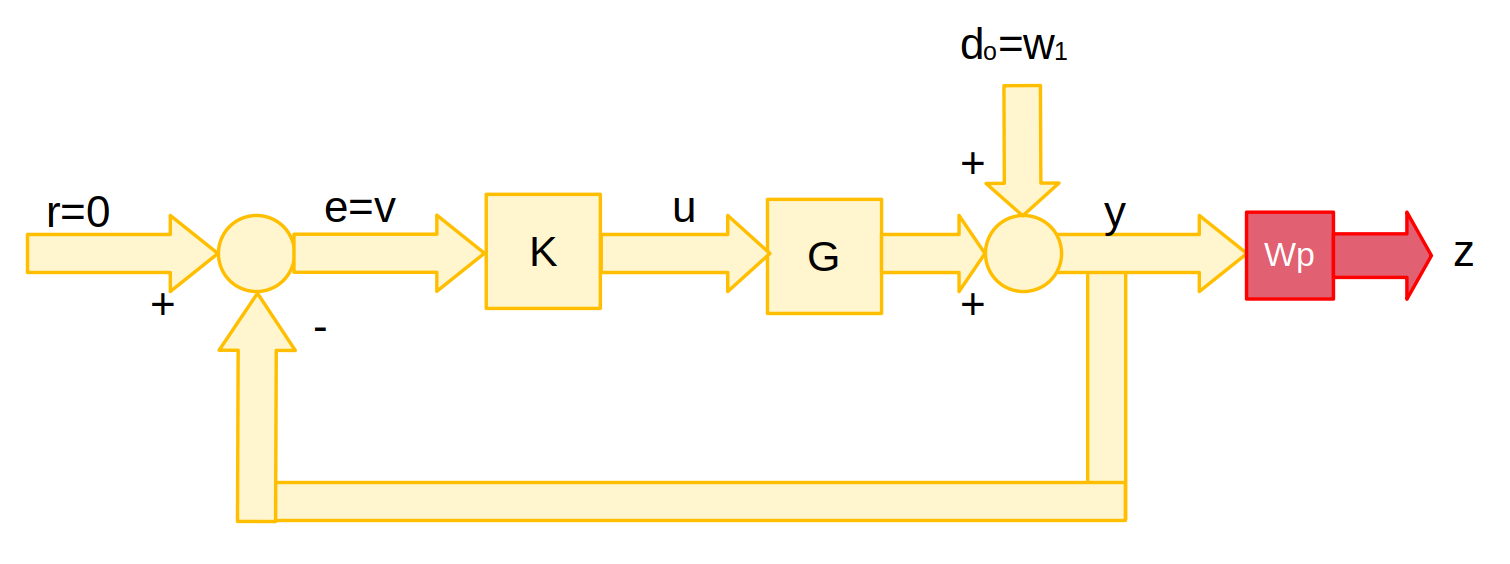
\includegraphics[width=\textwidth]{a4block.png}
\end{figure}

\subsection{}
\textit{Compute the generalized plant $P$ and close the lower LFT to compute the corresponding $w \to z$ transfer function and test for $H_\infty$ nominal performance.}

% Performance outputs and signals
The performance output and signals are defined as:
\[
\begin{aligned}
z &= W_p y = W_p (w + Gu), \\
v &= e = -y = -(w + Gu).
\end{aligned}
\]

% Generalized plant P
The generalized plant \(P\) is constructed as:
\[
\begin{bmatrix}
z \\
v
\end{bmatrix}
=
\begin{bmatrix}
W_p & W_p G \\
-I & -G
\end{bmatrix}
\begin{bmatrix}
w \\
u
\end{bmatrix}
\]

% Closed-loop transfer function F_l(P, K)
The closed-loop transfer function \(F_\ell(P, K)\) is derived as:
\[
\begin{aligned}
F_\ell(P, K) &= P_{11} + P_{12} K (I - P_{22} K)^{-1} P_{21}, \\
&= W_p + W_p G K (I + G K)^{-1} (-I), \\
&= W_p (I - T_O)
\end{aligned}
\]

% H_infinity performance criteria
The \(H_\infty\) performance criterion is:
\[
\| W_p S_0 \|_\infty < 1,
\]
where \(S_0 = (I + G K)^{-1}\) is the sensitivity function, and the transfer function from \(w \to z\) is \(T_O\).

\subsection{}
\textit{Assume a tracking performance weighting function of the form $W_p(s) = (s/M + \omega_B^*)/(s + \omega_B^* A) I$. Implement MATLAB code to synthesize a $H_\infty$ controller $K$ using either the \texttt{mixsyn} or \texttt{hinfyn} functions. Select design parameters $A$, $M$ and $\omega_B^*$ so that the resulting closed loop has a disturbance rejection capability of 10X and a closed loop bandwidth that is less than a 3 second rise time in each of the states.}

\begin{lstlisting}[style=matlabstyle]
A=0.05;
omegaB=1;
M=2;
s = tf('s');
Wp = (s/M+omegaB)/(s+omegaB*A)*eye(2);
W2=[];
W3=[];

[K,CL,GAM,INFO] = mixsyn(G,Wp,W2,W3);    
\end{lstlisting}

\subsection{}
\textit{When you have settled on a sufficient design, generate the following plots: (i) a comparison of the singular values of the plant $G$, the controller $K$ and the open loop transfer function matrix $GK$, (ii) verify that your system satisfies nominal performance by plotting the $|1/W_1(j\omega)|$ and $\hat{\sigma}(S_0)$ curves, (iii) the step response of the state $\beta$ for a unit step input in the $\delta_a$ and the step response of the state $r$ for a unit step input in the $\delta_r$, and (iv) the response of the $\beta$ state to a step in the first disturbance component $d_1$, and the response of the second state $r$ to a step in the second disturbance component $d_2$, where $d_o = [d_1\ d_2]^T$.}

\begin{figure}[H]
    \centering
    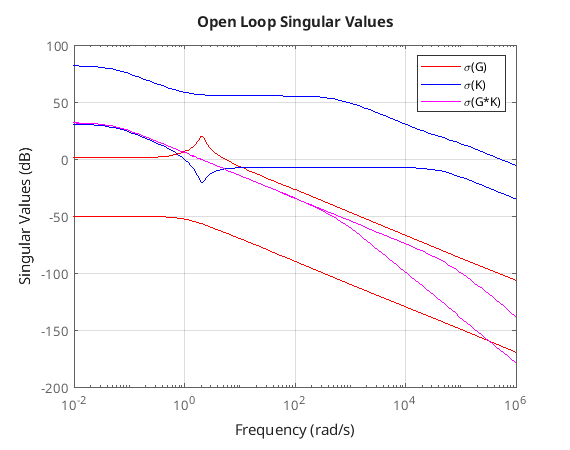
\includegraphics[width=\textwidth]{a4GKsigma.png}
\end{figure}

\begin{figure}[H]
    \centering
    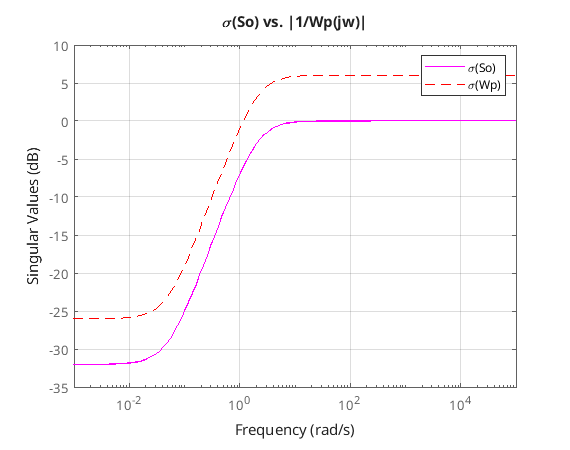
\includegraphics[width=\textwidth]{a4SoWp.png}
\end{figure}

\begin{figure}[H]
    \centering
    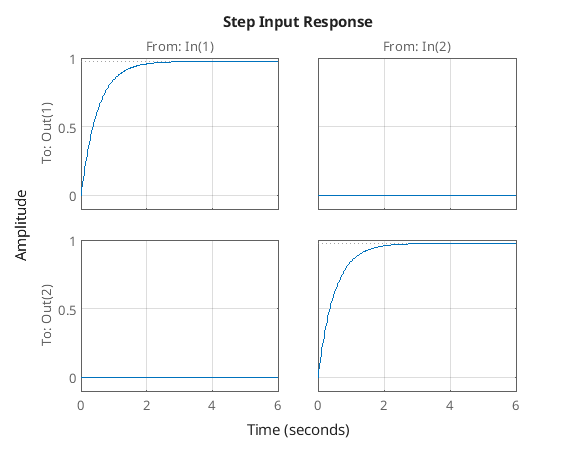
\includegraphics[width=\textwidth]{a4stepInput.png}
\end{figure}

\begin{figure}[H]
    \centering
    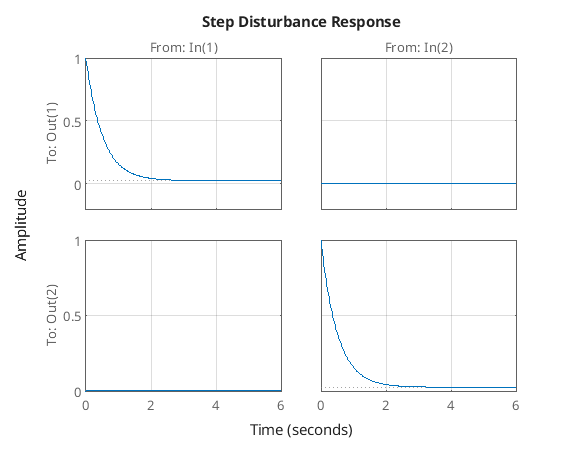
\includegraphics[width=\textwidth]{a4disturbance.png}
\end{figure}

\end{document}